\chapter{Cosmology Lecture 4: Homogeneity, Friedmann Dynamics, and the Equation of State}

This lecture begins by letting a string of questions do the real work. Before we write a cosmological field equation, we are forced to ask what expansion means, why ordinary bound systems do not simply fly apart, what homogeneity and isotropy mean mathematically, and how much our geometric intuition is corrupted by pictures of spaces embedded in something larger. Only after that clearing of the ground do we write the spacetime metric, give it dynamics, and finally ask what additional information is needed to determine the evolution of the scale factor.

\section{Opening Questions: Expansion, Size, and Conservation}

The lecture opens with a practical topological question: could the universe actually be smaller than the observable patch? The answer is cautious but firm. A small universe with periodic identifications would behave, in effect, like a torus: the same structures would repeat, and one would in principle see copies of the same astronomical patterns. The point is not that the idea is logically impossible, but that it has observable consequences. According to the lecture, people have looked for such periodicity and found no evidence for it, together with some evidence against it. In that sense the observable universe does not seem to be a repeated tiling of a smaller one.

A second question presses harder. If the universe expands, why do the solar system, atoms, and ordinary pieces of matter not expand along with it? Here Susskind insists that one must separate the cosmic tendency to separate distant comoving points from the local forces that bind matter.

\subsection{Question \& Answer}

\paragraph{Question.} How can an expanding universe coexist with stable atoms, solar systems, and with what we mean by energy conservation?

\paragraph{Answer.} Bound systems are held together by forces that are overwhelmingly stronger than the tiny tendency associated with cosmological expansion. If two people hold hands in space, the distance between them does not simply join the Hubble flow. The same is true, much more strongly, for atoms bound by electromagnetism and for planets bound by gravity. At most the expansion produces an utterly tiny perturbation; it does not tear these systems apart.

The energy-conservation question is subtler. In a static world, conservation of energy is tied to time-translation invariance. If the background itself is time dependent, that argument no longer goes through in the naive way. In an expanding universe the spacetime background changes with time, and the lecture explicitly warns that the familiar static-universe notion of global energy conservation is not the right one. Changes in energy are traded against the dynamics of expansion itself. This point is not yet the full formal statement of covariant conservation, but it is the motivation for the thermodynamic argument that will come later.

From here the lecture makes a crucial move. If we want to speak carefully about the universe as homogeneous and isotropic, we cannot remain at the level of slogans. We must say what those words mean for a metric.

\section{Homogeneity, Isotropy, and the Metric}

Susskind answers the next question geometrically, not dynamically. Einstein's equations describe how things change; homogeneity and isotropy are, first of all, statements about the structure of space.

\begin{definition}
A space is homogeneous if one can choose coordinates around any point in such a way that, after shifting the origin to any other point, the metric retains the same functional form. It is isotropic if, in addition, no direction at a given point is geometrically preferred.
\end{definition}

The cleanest example is flat space in two dimensions. Start with
\begin{align}
ds^2 &= dx_1^2 + dx_2^2 ,
\end{align}
and perform a translation of coordinates,
\begin{align}
y_1 &= x_1 + a_1, &
y_2 &= x_2 + a_2 .
\end{align}
Here the shift parameters \(a_1\) and \(a_2\) are only coordinate displacements; they have nothing to do with the cosmological scale factor. Differentiating gives \(dy_1=dx_1\) and \(dy_2=dx_2\), so the metric becomes
\begin{align}
ds^2 &= dy_1^2 + dy_2^2 .
\end{align}
Its form is unchanged. Therefore the neighborhood of one point is geometrically the same as the neighborhood of any translated point. That is homogeneity in its simplest form.

The sphere gives the next example. In the lecture the metric of the unit two-sphere is written in the form
\begin{equation}
d\Omega_2^2 = dr^2 + \sin^2 r\, d\theta^2 .
\end{equation}
If we choose the south pole as the origin, \(r\) is distance from that pole. If we instead rotate the sphere and choose a different pole, the explicit coordinate transformation is more complicated, but the point is that the metric takes exactly the same functional form in the new coordinates. Thus every point on the sphere is equivalent to every other point.

\subsection{Question \& Answer}

\paragraph{Question.} What do homogeneity and isotropy mean mathematically?

\paragraph{Answer.} Homogeneity means that one can move the origin from one point to another by a coordinate transformation and preserve the form of the metric. Isotropy means that around a given point no direction is singled out. These are statements about the geometry itself. They are not, at this stage, statements about the time evolution.

The lecture then inserts an important caveat: the torus. A torus with periodic identifications is translation invariant, so it is homogeneous in the sense just defined. But it is not isotropic. Certain directions are preferred by the identifications, and observations along one direction need not agree with those made along another. Thus homogeneity does not automatically imply isotropy.

There is also a scale issue. The universe is not homogeneous on small scales. Atoms, stars, galaxies, clusters, and large-scale density fluctuations all break perfect uniformity. Homogeneity is an averaged statement, meaningful only on sufficiently large scales. The lecture compares this to the surface of the Earth: mountains and valleys matter on small scales, but on large enough scales the surface is well approximated by a sphere. Cosmology uses the same kind of large-scale idealization.

\section{Intrinsic Geometry and the Trap of Embedding Pictures}

At this point the lecture pauses to dismantle a persistent source of confusion. When we say that space may be spherical, we do not mean that it is literally a balloon sitting inside a larger ambient space with an inside and an outside. The geometry relevant to physics is intrinsic. It is determined by measurements made within the space itself.

This is easiest to see in one dimension. A closed one-dimensional space can be drawn as a circle, as a square, or as a deformed peanut-shaped loop. From the intrinsic point of view, however, the drawing is not the geometry. What matters is the distance measured along the line. If two such closed one-dimensional spaces have the same circumference, then intrinsically they are the same geometry. The apparent bending of the drawing is only extrinsic.

\begin{figure}
\centering

\includegraphics[width=0.72\textwidth]{lecture_04_figure_05.png}
\caption{Round and deformed closed loops on the board. The point of the drawing is intrinsic, not pictorial: a one-dimensional closed space may be embedded in many ways while preserving the same internal geometry.}
\end{figure}

The lecture's claim is stronger still: one-dimensional spaces have no intrinsic curvature. Any small segment of a one-dimensional curve can be straightened without stretching it, so the apparent bending of a drawn line is not intrinsic curvature but only curvature of embedding.

\begin{remark}
A curved line on the page may have nonzero extrinsic curvature and yet zero intrinsic curvature. For a one-dimensional world, only the intrinsic geometry is visible to its inhabitants.
\end{remark}

A simple redraw makes the point in the cleanest possible way.

\begin{figure}
\centering
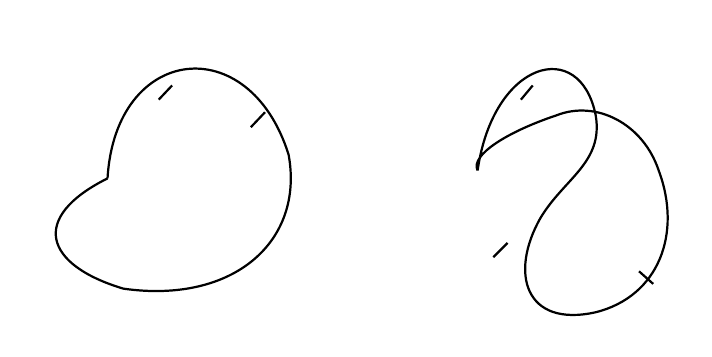
\begin{tikzpicture}[scale=1.0]
\draw[line width=0.8pt] (0,0) .. controls (0.1,1.7) and (1.8,1.9) .. (2.3,0.3)
  .. controls (2.5,-0.8) and (1.6,-1.6) .. (0.2,-1.4)
  .. controls (-0.8,-1.1) and (-1.0,-0.5) .. (0,0);
\draw[line width=0.8pt] (0.65,1.00) -- (0.82,1.18);
\draw[line width=0.8pt] (1.82,0.65) -- (2.00,0.84);

\draw[line width=0.8pt] (4.7,0.1) .. controls (4.9,1.5) and (6.0,1.8) .. (6.2,0.8)
  .. controls (6.3,0.2) and (5.8,0.0) .. (5.5,-0.5)
  .. controls (5.1,-1.2) and (5.3,-1.9) .. (6.2,-1.7)
  .. controls (7.0,-1.5) and (7.3,-0.7) .. (7.0,0.1)
  .. controls (6.8,0.7) and (6.2,1.0) .. (5.7,0.8)
  .. controls (5.1,0.6) and (4.6,0.3) .. (4.7,0.1);
\draw[line width=0.8pt] (5.25,1.00) -- (5.40,1.18);
\draw[line width=0.8pt] (5.08,-0.82) -- (4.90,-1.00);
\draw[line width=0.8pt] (6.75,-1.18) -- (6.93,-1.34);
\end{tikzpicture}
\caption{A clean redraw of the round and deformed one-dimensional closed spaces. If the distance around the loop is the same, the intrinsic geometry is the same.}
\end{figure}

The lecture then widens the lesson. A flat sheet of paper rolled into a cylinder is still intrinsically flat. A hemisphere cannot be flattened without stretching. That is the difference between extrinsic bending and intrinsic curvature. In this sense curvature is an intrinsic property, and in general relativity it measures tidal gravitational effects. That is why, when a student asks whether curvature implies gravity, the answer is yes: intrinsic curvature is a measure of tidal forces, and in the relativistic theory those forces are gravitational.

Only after this long warning does the lecture return to cosmology proper. The geometric possibilities we are about to write are intrinsic geometries, not pictures in a larger room.

\section{The FRW Ansatz and Hubble's Law}

Now the lecture is ready to accept the cosmological idealization. Space is taken to be homogeneous and isotropic on large scales, and therefore one of three kinds of geometry: positively curved, flat, or negatively curved. The symbol \(k\) labels the choice,
\[
k=+1,\qquad k=0,\qquad k=-1.
\]

The blackboard groups the possible spatial metrics under a single common factor \(a(t)^2\), the scale factor:

\begin{figure}
\centering

\includegraphics[width=0.74\textwidth]{lecture_04_figure_02.png}
\caption{Grouped spatial metrics and curvature labels. The board organizes the three spatial geometries under the common multiplier \(a(t)^2\).}
\end{figure}

The spacetime metric is then assumed to take the form
\begin{equation}
ds^2 = -dt^2 + a(t)^2\, d\Sigma_k^2 .
\end{equation}
The lecture emphasizes that this is already a nontrivial restriction: space and time are not mixed in the metric. Later, when a student asks whether that is an extra assumption, the answer is that it is forced by homogeneity and isotropy.

The three spatial metrics are
\begin{align}
d\Sigma_0^2 &= dx^2 + dy^2 + dz^2
            = dr^2 + r^2\, d\Omega_2^2, \\
d\Sigma_{+1}^2 &= d\Omega_3^2
               = dr^2 + \sin^2 r\, d\Omega_2^2, \\
d\Sigma_{-1}^2 &= dr^2 + \sinh^2 r\, d\Omega_2^2 .
\end{align}
At fixed time the geometry is therefore flat, spherical, or hyperbolic. What changes with time is the overall scale.

This immediately gives a kinematic derivation of Hubble's law. Let two galaxies sit at fixed comoving coordinates. Their coordinate separation is fixed, but their physical separation scales with \(a(t)\). If we call the fixed comoving separation \(\Delta\chi\), then
\begin{align}
D(t) &= a(t)\,\Delta\chi, \\
v(t) &= \dot a(t)\,\Delta\chi .
\end{align}
Dividing one by the other gives
\begin{equation}
v = \frac{\dot a}{a}\, D .
\end{equation}
The quantity \(\dot a / a\) may depend on time, but by construction it does not depend on position. That is the sense in which the Hubble parameter is spatially constant in the homogeneous model.

The lecture also makes a careful geometric remark about the meaning of \(a(t)\). In the positively curved case \(a(t)\) has a clean intrinsic meaning: it is the radius of the spatial three-sphere. In the flat case, where space is infinite, \(a(t)\) has no such invariant absolute meaning by itself; only ratios of scale factors or physical distances are observable.

\section{From Einstein's Equation to the Friedmann Equation}

Kinematics alone is not enough. Once the metric has been written, the next question is unavoidable: how does \(a(t)\) evolve? Here the lecture makes a methodological point that will matter all the way through cosmology. We cannot begin with Newton, because we are already talking about curved spacetime. We must begin with general relativity. Nevertheless the final equation will look strikingly Newtonian.

The lecture does not carry out the full Christoffel-symbol computation on the board. Instead it writes the structural form of Einstein's equation and then extracts the part of it that matters for cosmology.

\begin{figure}
\centering

\includegraphics[width=0.78\textwidth]{lecture_04_figure_03.png}
\caption{Einstein equation as written on the board. The visible frame clearly shows the geometric left-hand side and the prefactor \(8\pi G/3\).}
\end{figure}

In cleaned form we may write
\begin{equation}
R^{\mu\nu} - \frac12 g^{\mu\nu}R = \frac{8\pi G}{3}\, T^{\mu\nu}.
\end{equation}

\begin{remark}
The blackboard frame visibly stops at the prefactor \(8\pi G/3\). The appearance of \(T^{\mu\nu}\) is supplied by the transcript. The normalization is lecture-faithful here, even though it is not the usual textbook way of displaying the full tensor equation.
\end{remark}

The right-hand side contains the energy-momentum tensor. For the cosmological equation of immediate interest we focus on the time-time component, because
\begin{equation}
T_{00} = \rho .
\end{equation}
Thus the right-hand side becomes the energy density of whatever fills the universe.

The left-hand side is geometry. The lecture makes two structural claims about the time-time component. First, in the Einstein-tensor combination the terms with second derivatives cancel for the time-time component. Second, the surviving contributions split into a time-dependent part and a purely spatial-curvature part. The time-dependent part is proportional to \(\dot a^2/a^2\), and the spatial part is proportional to \(k/a^2\). That is enough to land on the Friedmann equation,
\begin{equation}
\left(\frac{\dot a}{a}\right)^2 + \frac{k}{a^2} = \frac{8\pi G}{3}\rho .
\end{equation}
The lecture then rewrites it in the more familiar form
\begin{equation}
\left(\frac{\dot a}{a}\right)^2 = \frac{8\pi G}{3}\rho - \frac{k}{a^2}.
\end{equation}

\subsection{Question \& Answer}

\paragraph{Question.} Why is the time-time component enough, and where did the second derivatives go?

\paragraph{Answer.} In the homogeneous and isotropic ansatz the only unknown function is \(a(t)\). Therefore one nontrivial Einstein equation is enough to determine the dynamics. The mixed space-time components vanish trivially in this ansatz, and the space-space equations are equivalent to the time-time equation up to the same dynamics. One can even form combinations that look like the Newtonian \(F=ma\) equation and contain \(\ddot a\). But in the time-time component, the special Einstein-tensor combination cancels the dangerous second-derivative terms, leaving the energy equation above.

This is the point at which the lecture draws the comparison with Newtonian cosmology. The equation is the same one we already met there. What changes is the interpretation of the curvature term. In the Newtonian story the corresponding constant was related to total energy and escape velocity. Here the same mathematical slot is occupied by the intrinsic curvature of space. The formal coincidence is not an accident: on sufficiently small patches of a curved universe, curvature becomes negligible and Newtonian motion must re-emerge.

At this stage the lecture also recalls the provisional relation between \(k\) and future evolution when the only forms of energy are matter and radiation. Positive \(k\) corresponds to the recollapsing case, negative \(k\) to the above-escape-velocity case, and \(k=0\) to the knife-edge case. But the lecture immediately warns that this simple correlation will fail once dark energy is admitted.

\section{Equation of State and Density Scaling}

The Friedmann equation is not yet an equation for \(a(t)\) alone. It still contains \(\rho\), and unless we know how \(\rho\) depends on \(a\), we cannot solve it. The lecture explicitly pauses here and says that this is the missing ingredient.

Before going general, Susskind recalls the two familiar examples. For ordinary nonrelativistic matter,
\begin{equation}
\rho_{\mathrm{matter}} = \frac{\rho_0}{a^3},
\end{equation}
and for radiation,
\begin{equation}
\rho_{\mathrm{rad}} = \frac{\rho_0}{a^4}.
\end{equation}
The board records these together with the equation of state:

\begin{figure}
\centering

\includegraphics[width=0.82\textwidth]{lecture_04_figure_06.png}
\caption{Equation of state with matter and radiation scalings. The lecture now shifts from named examples to the general relation \(P=w\rho\).}
\end{figure}

The general idea is encoded in the equation of state,
\begin{equation}
P = w\rho .
\end{equation}
For matter domination one has
\begin{equation}
w=0,
\end{equation}
because the particles are moving slowly and the pressure is negligible compared to the energy density. For radiation domination,
\begin{equation}
w=\frac13 .
\end{equation}
The lecture says explicitly that the factor \(1/3\) comes from three spatial dimensions, although the full derivation of that fact is postponed.

\begin{definition}
An equation of state is a relation between thermodynamic variables. In the present lecture it means a relation between pressure \(P\) and energy density \(\rho\), and the relevant class is \(P=w\rho\) with \(w\) constant.
\end{definition}

Now comes the worked derivation. Consider a box of material with volume \(V\), energy density \(\rho\), and total energy
\begin{equation}
E=\rho V .
\end{equation}
For slow adiabatic expansion the lecture keeps only the pressure-volume term,
\begin{equation}
dE=-P\,dV .
\end{equation}
On the other hand, differentiating \(E=\rho V\) gives
\begin{equation}
dE = \rho\, dV + V\, d\rho .
\end{equation}
Equating the two expressions for \(dE\), we get
\begin{align}
\rho\, dV + V\, d\rho &= -P\, dV, \\
V\, d\rho &= -(\rho+P)\, dV .
\end{align}
Now insert the equation of state \(P=w\rho\):
\begin{align}
V\, d\rho &= -(1+w)\rho\, dV .
\end{align}
Dividing by \(\rho V\) gives
\begin{equation}
\frac{d\rho}{\rho} = -(1+w)\frac{dV}{V}.
\end{equation}
The lecture recognizes both sides as logarithmic differentials,
\begin{equation}
d(\log \rho) = -(1+w)\, d(\log V),
\end{equation}
so after integration
\begin{equation}
\rho \propto V^{-(1+w)}.
\end{equation}
But for a comoving box in an expanding homogeneous universe,
\begin{equation}
V \propto a^3 .
\end{equation}
Therefore
\begin{equation}
\rho \propto a^{-3(1+w)},
\end{equation}
or more explicitly,
\begin{equation}
\rho = \frac{\text{const.}}{a^{3(1+w)}} .
\end{equation}

This immediately reproduces the two familiar cases:
\begin{align}
w=0 &\quad \Longrightarrow \quad \rho \propto a^{-3}, \\
w=\frac13 &\quad \Longrightarrow \quad \rho \propto a^{-4}.
\end{align}
The lecture now has a general framework in place: to describe a cosmological component, what we need to know is its equation of state.

At the very end Susskind opens the door to dark energy. Vacuum energy, dark energy, and the cosmological constant are identified here by a single parameter choice,
\begin{equation}
w=-1 .
\end{equation}
The same formula then gives
\begin{equation}
\rho \propto a^{0} = \text{constant}.
\end{equation}
That is the defining feature of vacuum energy in this lecture: when the universe expands, the energy density does not dilute. Empty space keeps the same energy density when stretched.

The lecture stops deliberately at this point. It notes that today the radiation energy density is tiny and is mostly the cosmic microwave background, whereas running backward in time makes the radiation component grow relative to matter. But the full analysis of the \(w=-1\) case and its consequences is postponed to the next lecture.

\section{Summary}

The lecture begins by forcing us to take seriously the questions that naive cosmological language invites. A small periodic universe would leave repeated images; bound systems do not simply join the cosmic expansion; and the usual static-world notion of global energy conservation does not survive unchanged in a time-dependent background.

From there the notes move to geometry. Homogeneity and isotropy are statements about the metric, not yet about dynamics, and they must be understood intrinsically rather than through pictures of embedded balloons and loops. With that conceptual ground cleared, the FRW metric
\[
ds^2=-dt^2+a(t)^2 d\Sigma_k^2
\]
follows naturally, together with the kinematic form of Hubble's law.

General relativity then supplies the dynamics. In the time-time component of Einstein's equation, the relevant combination reduces to the Friedmann equation,
\[
\left(\frac{\dot a}{a}\right)^2 = \frac{8\pi G}{3}\rho - \frac{k}{a^2},
\]
which is formally the same equation as in the Newtonian treatment, though the curvature term now has a genuinely geometric meaning.

Finally, the lecture identifies the remaining missing input: the dependence of \(\rho\) on \(a\). The equation of state \(P=w\rho\), together with the adiabatic identity \(dE=-P\,dV\), yields
\[
\rho \propto a^{-3(1+w)}.
\]
Matter and radiation reappear as \(w=0\) and \(w=1/3\), and the lecture closes with the teaser \(w=-1\), the case of dark energy, whose consequences are left for the next chapter.